\section{A Metric for Quantifying the Safety of Soft Robots}
Thereafter, we propose a quantitative safety metric that captures the particular characteristics that continuum soft robots exhibit (e.g., elasticity, actuation through their structure, Cosserat rod dynamics, etc.).
Importantly, the presented safety metric fulfills all the requirements that we laid out previously. % (e.g., based on a soft robotic dynamical model, computationally tractable, differentiable, etc.).
First, we state the necessary background on soft robotic dynamics and contact models. Subsequently, we derive the dynamics of a collision between the continuum soft robot and the human (body part).
Next, we propose two flavors of the safety metric: (i) the \textbf{Injury Severity Criterion (ISC)} captures the injury risk for a \emph{given} contact geometry, soft robot state, and actuation sequence. We envision this criterion to be useful for control applications with safety guarantees.
The second flavor, (ii) the \textbf{Design Hazardousness Criterion (DHC)}, captures the inherent safety of an integrated soft robot design (e.g., also considering the control policy) and leverages the \gls{ISC} for estimating the maximum injury risk over all possible contact geometries, feasible robot states and actuation sequences.
Apart from the procedure for formulating this safety metric, one of the key innovations here is that we identify a closed-form solution to the collision dynamics, which renders the computation of the \gls{ISC} to be computationally tractable.

\subsection{Background on Soft Robot Dynamics and Contact Model}
Following the Cosserat rod theory, we can capture the kinematic behavior of slender structures such as continuum soft robots by considering the deformations of the robot's backbone. As the 1D spatial deformations of this backbone are still an infinite-dimensional problem, the field has developed many methods (e.g., \gls{PCC}~\citep{webster2010design}, \gls{PCS}~\citep{renda2018discrete}, \gls{GVS}~\citep{renda2020geometric}, etc.) to describe such deformations with a finite number of finite vector of configuration variables $q \in \mathbb{R}^n$. The associated forward kinematic model then allows us to define the geometric positional Jacobian $J_\mathrm{p}(q, s) \in \mathbb{R}^{3 \times n}$, where $s \in [0,L]$ is the backbone abscissa/coordinate and $L$ is the length of the entire continuum structure.
Independent of the specific chosen kinematic model, the \gls{EOM} of a continuum soft robot can often be stated as~\citep{armanini2023soft, della2023model}
\begin{equation}\label{eq:safetymetric:soft_robot_configuration_space_dynamics}
    B(q) \, \ddot{q} + C(q, \dot{q}) \, \dot{q} + \partial_{q} \, \mathcal{U}(q) + D \, \dot{q} = A(q) \, u + \tau_\mathrm{c},
\end{equation}
$B(q) \in \mathbb{R}^{n \times n}$ and $C(q, \dot{q}) \in \mathbb{R}^{n \times n}$ considers the inertial and Coriolis effects of the soft robot system, respectively.
$\partial_{q} \, \mathcal{U}(q) \in \mathbb{R}^n$ captures the forces stemming from the potential $\mathcal{U}(q): \mathbb{R}^n \to \mathbb{R}$.
Often times, we the potential forces simplify to $\partial_{q} \, \mathcal{U}(q) =  G(q) + K q$, where $G(q) \in \mathbb{R}^{n}$ describes the gravitational forces, and $K \succ 0 \in \mathbb{R}^{n \times n}$ is the stiffness matrix.
Dissipation is integrated through the damping matrix $D \succ 0 \in \mathbb{R}^{n \times n}$.
$u(t,q,\dot{q}) \in \mathbb{R}^{m}$ contributes the actuation (determined by a control policy) that acts through the linear map $A(q) \in \mathbb{R}^{n \times m}$ on the generalized coordinates.

The term $\tau_\mathrm{c} \in \mathbb{R}^n$ collects all contributions by external contact forces on the generalized coordinates.
In the following, we will assume that the soft robot is only in contact with the human at one discrete point and that only pure forces are reflected between the bodies during the contact (i.e., no Cartesian torques).
Specifically, we assume that the contact occurs at a specific point $s_\mathrm{c}$ and that the contact exhibits a constant surface normal of $n_\mathrm{c} \in \mathcal{S}^3$ which is a unit vector and, with that, $\mathcal{S}^3 = \{ n_\mathrm{c} \in \mathbb{R}^3: \lVert n_\mathrm{c} \rVert_2 = 1 \}$.
We now describe with $\delta_\mathrm{c} > 0$ a penetration between the soft robot and the soft tissue of the human.
Then, the generalized torque acting on the soft robot as a consequence of the contact is given by $\tau_\mathrm{c} = -J^\top(q,s_\mathrm{c}) \, n_\mathrm{c} \, f_\mathrm{c}(\delta_\mathrm{c}, \dot{\delta}_\mathrm{c}) = -J_\mathrm{c}^\top(q) \, f_\mathrm{c}(\delta_\mathrm{c}, \dot{\delta}_\mathrm{c})$.
While the formulation that we use in this perspective for formulating the safety metric is compatible with many of the contact models that have been studied in the literature (e.g., Hunt-Crossley~\citep{hunt1975coefficient, aouaj2021predicting}, Hertz~\citep{johnson1987contact, park2011designing, she2020comparative}, etc.), we will mainly focus in the following on a linear spring-damper contact model~\citep{Isots_15066_2016, haddadin2009requirements} given by
\begin{equation}
    f_\mathrm{c}(\delta_\mathrm{c}, \dot{\delta}_\mathrm{c}) = \begin{cases}
        0 & \delta_\mathrm{c} \leq 0,\\
        k_\mathrm{c} \, \delta_\mathrm{c} + d_\mathrm{c} \, \dot{\delta}_\mathrm{c} & \delta_\mathrm{c} > 0,\\
\end{cases}
\end{equation}
where $k_\mathrm{c} \in \mathbb{R}_{>0}$ is the contact stiffness and $d_\mathrm{c} \in \mathbb{R}_{\geq 0}$ is the contact damping coefficient.
If we assume the soft robot surface material and the soft tissue to have spring constants and damping coefficients of $k_\mathrm{R,surf}$, $k_\mathrm{H,st}$ and $d_\mathrm{R}$, $d_\mathrm{H}$, respectively, then we can connect the spring-dampers in series
\begin{equation}
    k_\mathrm{c} = \left (\frac{1}{k_\mathrm{R,surf}} + \frac{1}{k_\mathrm{H,st}} \right )^{-1},
    \qquad
    d_\mathrm{c} = \left (\frac{1}{d_\mathrm{R}} + \frac{1}{d_\mathrm{H}} \right )^{-1}.
\end{equation}

\subsection{Collision Dynamics}
We now progress towards a formulation of the collision dynamics as motions of the soft robot and the human body part along the contact surface normal $n_\mathrm{c}$.

First, we describe the motion of the contact point of the soft robot with position and velocity $x_\mathrm{R}, \dot{x}_\mathrm{R} \in \mathbb{R}$.
We can project the dynamics of \eqref{eq:safetymetric:soft_robot_configuration_space_dynamics} into this 1D motion through the expression $\dot{x}_\mathrm{R} = J_\mathrm{c} \, \dot{q}$ yielding the form~\citep{khatib1987unified, della2019exact, della2020model, stolzle2024guiding}
\begin{equation}
    \Lambda_\mathrm{c}(q) \, \Ddot{x}_\mathrm{R} + \mu_\mathrm{c}(q,\dot{q}) \, \dot{x}_\mathrm{R} + J_\mathrm{c,B}^{+\top}(q) ( \partial_{q} \, \mathcal{U}(q) + D \dot{q} ) = J_\mathrm{c,B}^{+\top}(q) \, A(q) \, u - f_{\mathrm{c}}(\delta_\mathrm{c}, \dot{\delta}_\mathrm{c}),
\end{equation}
where $J_\mathrm{c,B}^{+\top}(q) = J_\mathrm{B}^+(q,s_\mathrm{c},n_\mathrm{c}) = B^{-1}J_\mathrm{c}^\top(J_\mathrm{c} B^{-1} J_\mathrm{c}^\top)^{-1} \in \mathbb{R}^{n \times 1}$ is the dynamically consistent pseudo-inverse, $\Lambda_\mathrm{c}(q) = \Lambda(q,s_\mathrm{c},n_\mathrm{c}) = (J_\mathrm{c} \, B^{-1} J_\mathrm{c}^\top)^{-1} \in \mathbb{R}^{1 \times 1}$ is the reflected inertia of the soft robot at the contact point~\citep{haddadin2009requirements, Isots_15066_2016}, and $\mu_\mathrm{c}(q,\dot{q}) = \mu(q, \dot{q},s_\mathrm{c},n_\mathrm{c}) = \Lambda(q) \, (J_\mathrm{c} B^{-1} C - \dot{J}_\mathrm{c}) \in \mathbb{R}^{1 \times n}$ collects the Cartesian Coriolis and centrifugal terms~\citep{khatib1987unified}.
If not explicitly stated otherwise, we will in the following, to simplify the notation, drop the specific dependency on the contact geometry $(s_\mathrm{c}, n_\mathrm{c})$: $J_\mathrm{c,B}^{+\top}(q) = J_\mathrm{B}^{+\top}(q,s_\mathrm{c},n_\mathrm{c})$, $\Lambda_\mathrm{c}(q) = \Lambda(q,s_\mathrm{c},n_\mathrm{c})$, etc.

Next, we move towards modeling the behavior of the human body part. In literature, the human body part is usually modeled as a point mass $m_\mathrm{H}$~\citep{haddadin2011safe, Isots_15066_2016} that moves in 1D along the surface normal of the contact with state $(x_\mathrm{H},\dot{x}_\mathrm{H})$. Instead, we take here a conservative approach and assume that the human body is constrained in its motion with velocity $v_\mathrm{H} \in \mathbb{R}$ towards the soft robots (i.e., $m_\mathrm{H} \gg \Lambda(q) \: \forall q$). This represents the \emph{worst case}.
After the coordinate change $\delta_\mathrm{c}(t) = x_\mathrm{R}(t) - x_\mathrm{H}$, $\dot{\delta}_\mathrm{c} = \dot{x}_\mathrm{R}(t) + v_\mathrm{H}$, % where $x^{\mathrm{c}0} \in \mathbb{R}$ is the position of the initial contact, 
where $x_\mathrm{H} \in \mathbb{R}$ is the position of the soft tissue surface, and while only considering the case of contact (i.e., $\delta_\mathrm{c} \geq 0$), the collision dynamics are given by
\begin{equation}
    \Lambda_\mathrm{c}(q) \, \Ddot{\delta}_\mathrm{c} + \mu_\mathrm{c}(q,\dot{q}) \, \dot{\delta}_\mathrm{c} + J_\mathrm{c,B}^{+\top}(q) ( \partial_{q} \, \mathcal{U}(q) + D \dot{q} ) = J_\mathrm{c,B}^{+\top}(q) \, A(q) \, u - k_\mathrm{c} \, \delta_\mathrm{c} - d_\mathrm{c} \, \dot{\delta}_\mathrm{c}.
\end{equation}
We are now interested in identifying the maximum force $f_\mathrm{c}(t)$ that occurs during the entire collision of the contact.
Therefore, we can neglect any damping forces as they dissipate energy.
Furthermore, we assume that the Coriolis effects are sufficiently small and can be neglected as well.
Finally, we assume that the change of configuration during the collision is sufficiently small such that the dynamic matrices can be approximated as constant: $m_\mathrm{R} \approx \Lambda_\mathrm{c}(q^{\mathrm{c}0})$, 
$A_\mathrm{c} \approx J_\mathrm{c,B}^{+\top}(q^{\mathrm{c}0}) \, A(q^{\mathrm{c}0})$, where the $q^{\mathrm{c}0}$ is the configuration of the robot at the beginning of the contact.
The same assumption also allows us to linearize the potential forces of the soft robot with 
\begin{equation}
    f_\mathcal{U} = J_\mathrm{c,B}^{+\top}(q) \, \partial_{q} \, \mathcal{U}(q) \approx \underbrace{J_\mathrm{c,B}^{+\top}(q^{\mathrm{c}0}) \, \partial_{q} \, \mathcal{U}(q^{\mathrm{c}0})}_{f_\mathcal{U}^{\mathrm{c0}}} + \underbrace{\frac{\partial}{\partial q} J_\mathrm{c,B}^{+\top}(q) \, \partial_{q} \, \mathcal{U}(q) \Big |_{q=q^{\mathrm{c}0}} \,  J_\mathrm{c,B}^{+}(q^{\mathrm{c}0})}_{k_\mathrm{R}}  \, \delta_\mathrm{c},
\end{equation}
where $k_\mathrm{R} \in \mathbb{R}$ is the local stiffness of the system against small perturbations and $f_\mathcal{U}^{\mathrm{c0}}$ are the potential forces present at the start of the contact.
Integrating the stated assumptions results in the approximated collision dynamics
\begin{equation}\label{eq:safetymetric:simplified_collision_dynamics}
    m_\mathrm{R} \, \Ddot{\delta}_\mathrm{c} + (k_\mathrm{R} + k_\mathrm{c}) \, \delta_\mathrm{c} = f_u - f_\mathcal{U}^{\mathrm{c0}}.
\end{equation}
To avoid computationally expensive simulations of the collision, we identify a closed-form solution to the collision dynamics
\begin{equation}\small\label{eq:safetymetric:collision_dynamics_cfs}
\begin{split}
    \delta_\mathrm{c}(t) =& \: \left (\delta_\mathrm{c}^0-\frac{f_u-f_\mathcal{U}^{\mathrm{c0}}}{k_\mathrm{R} + k_\mathrm{c}} \right ) \cos \left ( \sqrt{\frac{k_\mathrm{R} + k_\mathrm{c}}{m_\mathrm{R}}} \, t \right ) + \dot{\delta}_\mathrm{c}^0 \sqrt{\frac{m_\mathrm{R}}{k_\mathrm{R} + k_\mathrm{c}}} \, \sin \left ( \sqrt{\frac{k_\mathrm{R} + k_\mathrm{c}}{m_\mathrm{R}}} \, t \right ) + \frac{f_u-f_\mathcal{U}^{\mathrm{c0}}}{k_\mathrm{R} + k_\mathrm{c}},\\
    % \dot{\delta}_\mathrm{c}(t) =& \: -\sqrt{\frac{k_\mathrm{R} + k_\mathrm{c}}{m_\mathrm{R}}} \left (\delta_\mathrm{c}^0 - \frac{f_u-f_\mathcal{U}^{\mathrm{c0}}}{k_\mathrm{R} + k_\mathrm{c}} \right ) \, \sin \left ( \sqrt{\frac{k_\mathrm{R} + k_\mathrm{c}}{m_\mathrm{R}}} \, t \right ) + \dot{\delta}_\mathrm{c}^0 \, \cos \left ( \sqrt{\frac{k_\mathrm{R} + k_\mathrm{c}}{m_\mathrm{R}}} \, t \right ),
\end{split}
\end{equation}
where we assume without loss of generality that $t=0$ at the start of the collision, and $\delta_\mathrm{c}^0$ is the initial penetration depth.
The initial penetration velocity can be computed as a function of the configuration-space velocity as $\dot{\delta}_\mathrm{c}^0 = J_\mathrm{c}(q^{\mathrm{c}0}) \, \dot{q}^{\mathrm{c}0} + v_\mathrm{H}$.
Furthermore, we assume the actuation force to be constant, which can be easily accomplished by conservatively considering the maximum actuation force $f_u = \max_t A_\mathrm{c} \, u(t)$ that the robot experiences during the collision.

\begin{figure}[h!]
    \centering
    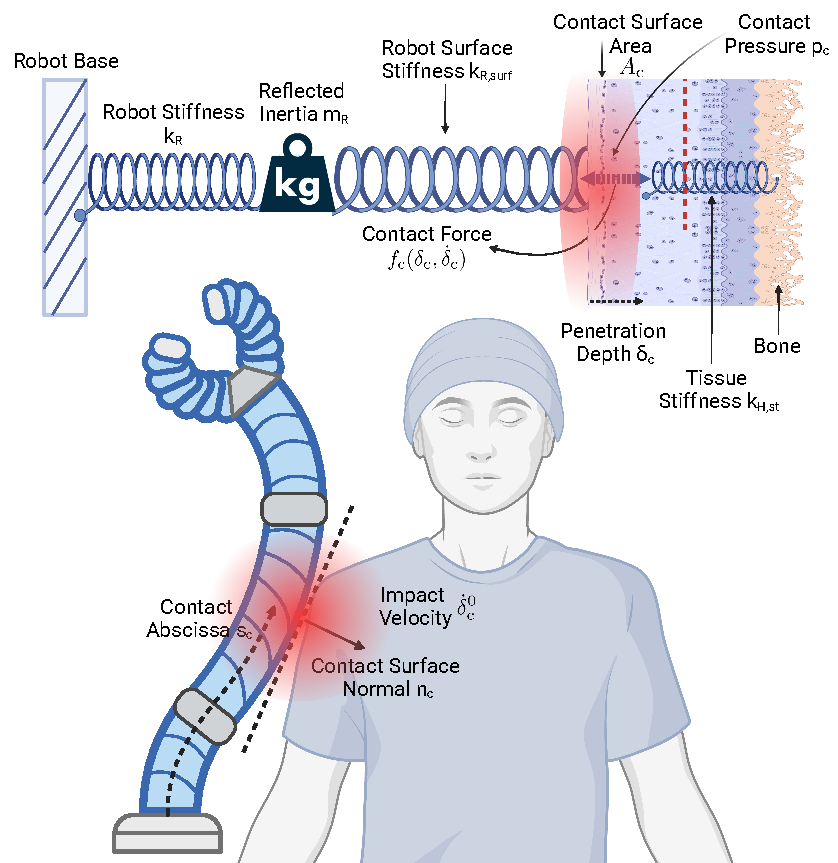
\includegraphics[width=0.9\linewidth]{safetymetric/figures/injury_severity_criterion.pdf}
    \caption{Proposed \emph{Injury Severity Criterion} as a safety metric for soft robots: The maximum contact pressure $\max_t p_\mathrm{c}(t) = \max_t \frac{f_\mathrm{c}(t)}{A_\mathrm{c}}$ experienced during the (potential) collision acts as a proxy for the expected injury risk~\citep{Isots_15066_2016}, where $f_\mathrm{c}(t)$ denotes the contact force and $A_\mathrm{c}$ the contact area. For computing $f_\mathrm{c}(t)$, we derive the dynamics of the collision (i.e., the time evolution of the penetration depth $\delta_\mathrm{c}(t))$ by projecting the dynamics of the soft robot onto a 1D Cartesian motion along the contact surface normal. In order to get a conservative estimate of the injury risk, we assume the human body part to be constrained in its motion (i.e., that the inertia of the human body part dominates the reflected inertia of the soft robot $m_\mathrm{R}$).}
    \label{fig:safetymetric:injury_severity_criterion}
\end{figure}

\subsection{Injury Severity Criterion}
Following the standards established in ISO/TS 15066:2016~\citep{Isots_15066_2016}, we consider the maximum contact pressure experienced during the collision as a proxy for the injury risk. Therefore, we define the \emph{Injury Severity Criterion} for a given tuple $(q^{\mathrm{c}0},s_\mathrm{c}, n_\mathrm{c})$ capturing the contact geometry as
\begin{equation}
    \mathrm{ISC}(q^{\mathrm{c}0},\dot{\delta}_\mathrm{c}^0,u,s_\mathrm{c},n_\mathrm{c}) = \max_t p_\mathrm{c} = \max_t \frac{f_\mathrm{c}(t)}{A_\mathrm{c}(t)} \leq \frac{\max_t f_\mathrm{c}(t)}{\min_t A_\mathrm{c}(t)} =  \frac{k_\mathrm{c} \max_t \delta_\mathrm{c}(t)}{\min_t A_\mathrm{c}(t)},
\end{equation}
where $p_\mathrm{c}(t)$ is the contact pressure, and $A_\mathrm{c}$ is the contact area.

The closed-form solution to the collision dynamics of \eqref{eq:safetymetric:collision_dynamics_cfs} allows us to upper-bound the maximum contact force $\max_t f_\mathrm{c}(t)$ that is encountered during the collision as
\begin{equation}
     \max_{t}f_\mathrm{c}(t) = k_\mathrm{c} \, \left ( \frac{f_u-f_\mathcal{U}^{\mathrm{c0}}}{k_\mathrm{R} + k_\mathrm{c}} + \sqrt{\left ( \delta_\mathrm{c}^0 - \frac{f_u-f_\mathcal{U}^{\mathrm{c0}}}{k_\mathrm{R} + k_\mathrm{c}} \right )^2 + \left (\dot{\delta}_\mathrm{c}^0 \right )^2 \frac{m_\mathrm{R}}{k_\mathrm{R} + k_\mathrm{c}} } \right ).
\end{equation}

% \subsubsection{Example: Mass-Spring Robot}
% First, we consider the most \emph{basic} soft robot - a damped mass-spring system with dynamics $m_\mathrm{R} \, \ddot{q} + k_\mathrm{R} \, (q-q^0) + d_\mathrm{R} \, \dot{q} = u + \tau_\mathrm{c}$, where $q \in \mathbb{R}$ and $q^0$ is the equilibrium extension. The \emph{Injury Severity Criterion} is then given by
% \begin{equation}
%      \mathrm{ISC} = \frac{k_\mathrm{c}}{A_\mathrm{c}} \, \left (\frac{u - k_\mathrm{R} (q^{\mathrm{c}0} - q^0)}{k_\mathrm{R} + k_\mathrm{c}} + \sqrt{\left ( \delta_\mathrm{c}^0 - \frac{u - k_\mathrm{R} (q^{\mathrm{c}0} - q^0)}{k_\mathrm{R} + k_\mathrm{c}} \right )^2 + \left (\dot{\delta}_\mathrm{c}^0 \right )^2 \frac{m_\mathrm{R}}{k_\mathrm{R} + k_\mathrm{c}} } \right ),
% \end{equation}
% with the limit $\lim_{k_\mathrm{R} \to \infty} \mathrm{ISC} = 2 \, \frac{k_\mathrm{c}}{A_\mathrm{c}} \left ( q^{\mathrm{c}0} - q^0 \right )$ for $\delta_\mathrm{c}^0 = 0$. 

\subsubsection{Example: Planar Piecewise Constant Strain Robot}
1 Figure giving an example how the contact location influences the injury severity.
\begin{itemize}
    \item Variation of injury severity for various contact geometries (e.g., various locations along the backbone, various contact surface normal) and configurations.
    \item Variation across model discretization granularity.
\end{itemize}

\subsubsection{Example: Integrating a Control Policy}
% alternative heading: \subsection{Influence of Control Policy}
An important question when analyzing the safety of a closed-loop soft robotic system is what influence the control policy has on the \gls{ISC}.
First, we consider a case where the behavior of the control policy $u = \phi(q,\dot{q})$ cannot be bounded or even inspected, such as it would be the case for controllers that contain integral terms or for many RL-based control policies.
In this case, access to actuation bounds $[u_\mathrm{min}, u_\mathrm{max}]$ provides us with the injury risk in the \emph{worst case scenario}.

Next, we consider the example of a \emph{PD+Feedforward}-like control structure that is relevant for many control policies that involve feedforward and/or feedback terms.
Specifically, we consider a fully-actuated setting (i.e., $n=m$) with an identity actuation matrix $A(q) = \mathbb{I}^n$.
Then, a regulator $\phi(q,\dot{q}) = \partial_{q} \, \mathcal{U}( q^\mathrm{d}) + K_\mathrm{p} \, (q^\mathrm{d}-q) - K_\mathrm{d} \, \dot{q}$ drives the system towards the setpoint $q^\mathrm{d}$~\citep{della2023model} and establishes the closed-loop dynamics
\begin{equation}
    B(q) \, \ddot{q} + C(q, \dot{q}) \, \dot{q} + \partial_{q} \, \mathcal{U}(q) + K_\mathrm{p} \, q + (D+K_\mathrm{d}) \, \dot{q} = \partial_{q} \, \mathcal{U}( q^\mathrm{d}) + K_\mathrm{p} \, q^\mathrm{d} + \tau_\mathrm{c},
\end{equation}
where $K_\mathrm{p}, K_\mathrm{d} \in \mathbb{R}^{n \times n}$ are the proportional and derivative feedback gains, respectively.
When re-formulating the simplified collision dynamics of \eqref{eq:safetymetric:simplified_collision_dynamics}, 
\begin{equation}
    m_\mathrm{R} \, \Ddot{\delta}_\mathrm{c} + (k_\mathrm{R} + k_\mathrm{c}) \, \delta_\mathrm{c} = J_\mathrm{c,B}^{+}(q^{\mathrm{c}0}) \, (\partial_{q} \, \mathcal{U}(q^\mathrm{d}) +  K_\mathrm{p} \, q^\mathrm{d} - \partial_{q} \, \mathcal{U}(q^{\mathrm{c}0})).
\end{equation}
We notice that the feedforward control term acts through a constant force on the oscillatory system.
The proportional feedback term increases the local stiffness of the robot: $k_\mathrm{R} = \frac{\partial}{\partial q} J_\mathrm{c,B}^{+\top}(q) \, \left ( \partial_{q} \, \mathcal{U}(q) + K_\mathrm{p} \, q \right )\Big |_{q=q^{\mathrm{c}0}} \,  J_\mathrm{c,B}^{+}(q^{\mathrm{c}0})$.
This analysis agrees with similar results known in literature~\citep{della2017controlling}.

\subsection{Design Hazardousness Criterion}
As presented in Fig.~\ref{fig:safetymetric:safety_metric_applications}, one application of a soft robotic safety metric would be to answer the question "\emph{How safe is this proposed soft robot design?}". The \gls{ISC} on its own is not sufficient to answer this question as it relies on a knowledge of the soft robot state at the beginning of the collision $(q^{\mathrm{c}0}, \dot{q}^{\mathrm{c}0})$, and the contact geometry $(s_\mathrm{c},n_\mathrm{c})$.
Therefore, we define the \gls{DHC} as the maximum injury severity that can be imposed by the soft robot over all feasible soft robot states, all possible contact geometries, and actuation sequences
\begin{equation}
\begin{split}
    \mathrm{DHC} =& \: \max_{q \in \mathcal{Q}} \max_{\dot{\delta}_\mathrm{c}^0 \in [0,\dot{\delta}_\mathrm{c}^\mathrm{max}]} \max_{u \in [u_\mathrm{min}, u_\mathrm{max}]} \max_{s_\mathrm{c} \in [0,L]} \max_{n_\mathrm{c} \in \mathcal{S}^3} \mathrm{ISC}(q^{\mathrm{c}0},\dot{\delta}_\mathrm{c}^0,u,s_\mathrm{c},n_\mathrm{c}),\\
    \leq& \: \max_{q \in \mathcal{Q}} \max_{s_\mathrm{c} \in [0,L]} \max_{n_\mathrm{c} \in \mathcal{S}^3} \mathrm{ISC}(q^{\mathrm{c}0},\dot{\delta}_\mathrm{c}^\mathrm{max},\lVert u_\mathrm{max} \rVert_2,s_\mathrm{c},n_\mathrm{c}),
\end{split}
\end{equation}
where $\mathcal{Q}$ is the set of feasible soft robot configurations.
To make this optimization more tractable, we can leverage the stated upper bound with $\dot{\delta}_\mathrm{c}^\mathrm{max} = \lVert J_\mathrm{c} \rVert_2 \, \lVert \dot{q}_\mathrm{max} \rVert_2 + v_\mathrm{H}$
and $f_u^\mathrm{max} = \lVert A_\mathrm{c} \rVert_2 \, \lVert \max(|u_\mathrm{min}|,|u_\mathrm{max}|) \rVert_2$.
We note that the maximum value of $\dot{q}_\mathrm{max}$ that the robot can achieve autonomously is, in practice, often given by certain actuator characteristics (e.g., maximum servo velocity for tendon-driven actuation).